%%
%% Author: anju s
%% 
%% Tables and figures required for my thesis.
%%

\NeedsTeXFormat{LaTeX2e}
\ProvidesPackage{thesisfiguresandtables} [2012/01/05]


\def\figgraphmatrices{
  \begin{figure}[htbp]% [t] % [p]%
    \centering

  \begin{tabular}[htbp]{cccl}
    \figtabsize
    ${\bf G_1}$: 
    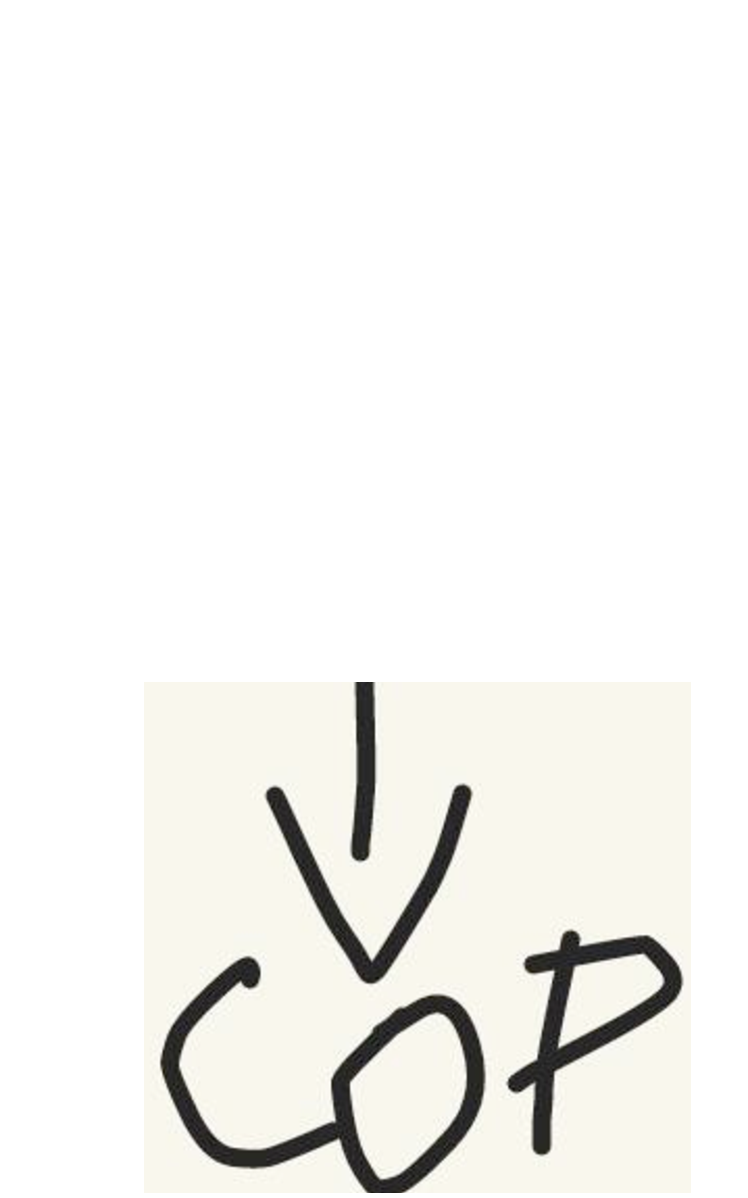
\includegraphics[scale=0.2]{../img/ex1_concaveroundgr.pdf} &
    ${\bf G_2}$: 
    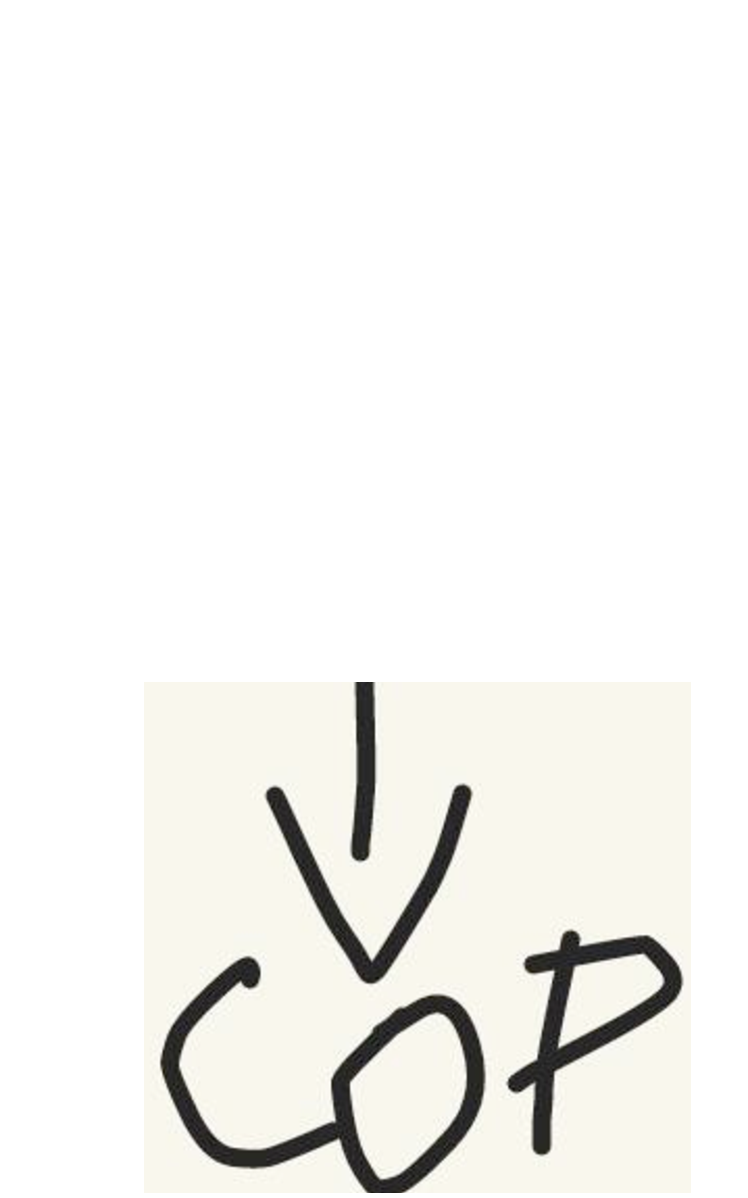
\includegraphics[scale=0.2]{../img/ex2_intervalgr.pdf} &
    ${\bf H}$: 
    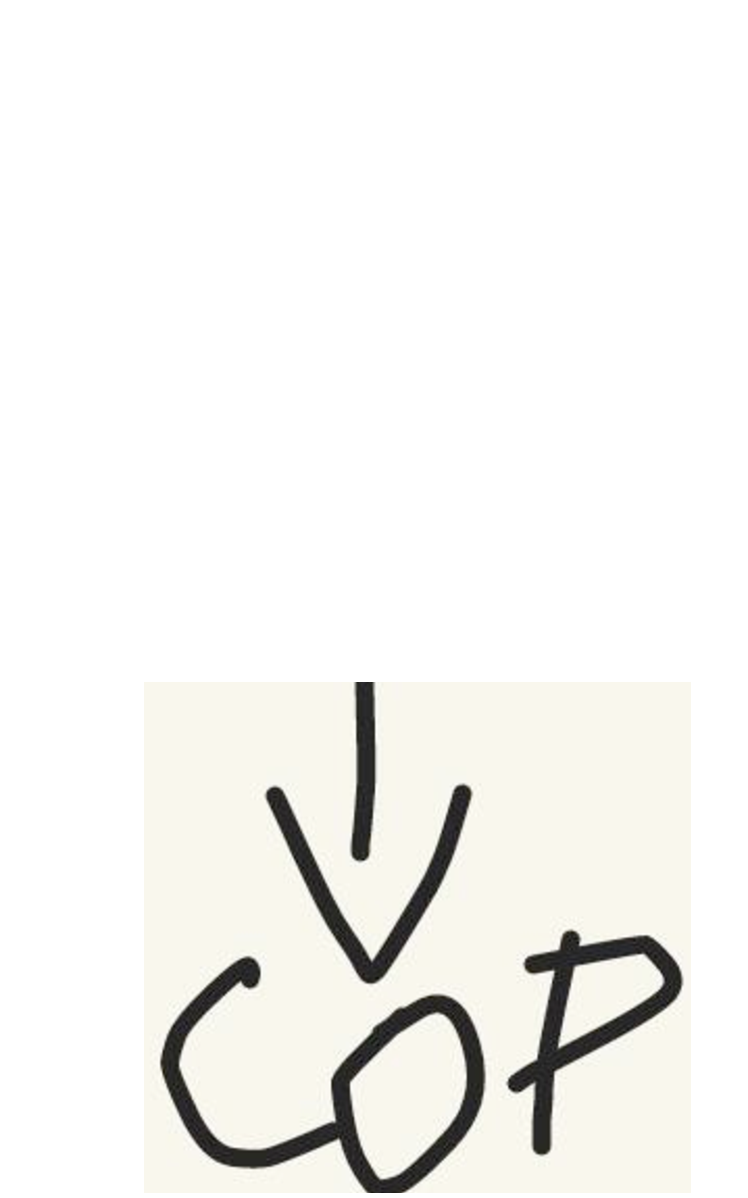
\includegraphics[scale=0.2]{../img/ex2_intervalgr.pdf} &
    \begin{tabular}[htbp]
      {>{\columncolor{\tblhcolor}}  l llll}                       % Shade header col..
      \rowcolor[gray]{0.8} 
      ${\bf C}$ &$w_1$ &$w_2$ &$w_3$ &$w_4$\\ % ..and row
      % \hline
      $u_1$ &\un   &\un   &0     &0   \\
      $u_2$ &\un   &\un   &\un   &\un \\
      $u_3$ &0     &0     &\un   &\un \\
      $u_4$ &0     &\un   &\un   &0   \\
      $u_5$ &\un   &\un   &\un   &0   
    \end{tabular}
  \end{tabular}\\
  \vspace{5mm}
  \begin{tabular}{lll}
    \begin{tabular}[htbp]%{l|lll lll}
      {>{\columncolor{\tblhcolor}}  l llllll}                       % Shade header col..
      \rowcolor[gray]{0.8}                                          % ..and row
      ${\bf A_1}$ &$v_1$ &$v_2$ &$v_3$ &$v_4$ &$v_5$ &$v_6$\\
      % \hline
      $v_1$     &0     &\un   &\un  &0     &\un   &\un \\
      $v_2$     &\un   &0     &\un  &\un   &0     &\un \\
      $v_3$     &\un   &\un   &0    &\un   &\un   &0   \\
      $v_4$     &0     &\un   &\un  &0     &0     &0   \\
      $v_5$     &\un   &0     &\un  &0     &0     &0   \\
      $v_6$     &\un   &\un   &0    &0     &0     &0   
    \end{tabular}
    & 
    \begin{tabular}[htbp]
      {>{\columncolor{\tblhcolor}}  l llll}                       % Shade header col..
      \rowcolor[gray]{0.8}                                          % ..and row
      ${\bf B}$&$c_1$ &$c_2$ &$c_3$ &$c_4$\\
      % \hline
      $v_1$ &\un   &\un   &\un   &0   \\
      $v_2$ &\un   &0     &0     &0   \\
      $v_3$ &0     &\un   &0     &0   \\
      $v_4$ &0     &0     &\un   &\un \\
      $v_5$ &0     &\un   &\un   &0   \\
      $v_6$ &0     &0     &0     &\un  
    \end{tabular}
    & 
    \\    
    && \\
    \begin{tabular}[htbp]
      {>{\columncolor{\tblhcolor}}  l llllll}                       % Shade header col..
      \rowcolor[gray]{0.8}                                          % ..and row
      ${\bf A_2}$&$v_1$ &$v_2$ &$v_3$ &$v_4$ &$v_5$ &$v_6$\\
      % \hline
      $v_1$ &\un   &\un   &\un  &0     &\un   &\un \\
      $v_2$ &\un   &\un   &\un  &\un   &0     &\un \\
      $v_3$ &\un   &\un   &\un  &\un   &\un   &0   \\
      $v_4$ &0     &\un   &\un  &\un   &0     &0   \\
      $v_5$ &\un   &0     &\un  &0     &\un   &0   \\
      $v_6$ &\un   &\un   &0    &0     &0     &\un 
    \end{tabular}    
    &
    \begin{tabular}[htbp]
      {>{\columncolor{\tblhcolor}}  l llllll}                       % Shade header col..
      \rowcolor[gray]{0.8}                                          % ..and row
      ${\bf A_2'}$ &$v_1$ &$v_6$ &$v_2$ &$v_4$ &$v_3$ &$v_5$\\
      % \hline
      $v_1$ &\un   &\un   &\un  &0     &\un   &\un \\
      $v_6$ &\un   &\un   &\un  &0     &0     &0   \\
      $v_2$ &\un   &\un   &\un  &\un   &\un   &0   \\
      $v_4$ &0     &0     &\un  &\un   &\un   &0   \\
      $v_3$ &\un   &0     &\un  &\un   &\un   &\un \\
      $v_5$ &\un   &0     &0    &0     &\un   &\un 
    \end{tabular}
    & \\
  \end{tabular}

  \caption[\figtabsize Matrices defined in
  Def.~\ref{def:graphmatrices}]{\figtabsize $A_1$ is the {\em
      adjacency matrix} and $A_2$ is the {\em augmented adjacency
      matrix} of $G_1$. $A_2'$ is obtained from $A_2$ by permuting its
    rows and columns to achieve {\em \CROP order}, \ie $A_2$ has
    \CROP\,-- thus $G_1$ is {\em a concave-round graph}
    (Def.~\ref{def:graphwithcop}~\ref{def::concave-round}) and {\em a
      circular-arc graph} (Tab.~\ref{tab:graphmatrices}) $B$ is the
    maximal clique matrix of $G_2$ and has \COP\,-- thus $G_2$ is an
    {\em interval
      graph}(Def.~\ref{def:graphwithcop}~\ref{def::concave-round}). $C$
    is the half adjacency matrix of bipartite graph $H$ and has \COP
    on rows -- thus $H$ is {a convex bipartite graph}.}
  \label{fig:graphmatrices}
  \end{figure}
}
